%\todo[inline]{Brug \textbackslash todo\{\} til ting der mangler %at blive lavet.\newline
%Brug \textbackslash unsure\{\} til ting i er usikre på om er %korrekte.\newline
%Brug \textbackslash change\{\} til ting der helt sikkert skal %ændres.\newline
%Brug \textbackslash info\{\} til generel info (useless).\newline
%Brug \textbackslash improvement\{\} til at foreslå forbedringer.}

\documentclass[a4paper,11pt,fleqn,twoside,openright]{memoir} 	% Openright aabner kapitler paa hoejresider (openany begge)
%%%% PACKAGES %%%%
\usepackage{amsmath}

% ¤¤ Oversaettelse og tegnsaetning ¤¤ %
\usepackage[utf8]{inputenc}					% Input-indkodning af tegnsaet (UTF8)
\usepackage[english]{babel}					% Dokumentets sprog
\usepackage[T1]{fontenc}					% Output-indkodning af tegnsaet (T1)
\usepackage{ragged2e,anyfontsize}			% Justering af elementer
%\usepackage{fixltx2e}						% Retter forskellige fejl i LaTeX-kernen
																			
% ¤¤ Figurer og tabeller (floats) ¤¤ %
\usepackage{graphicx} 						% Haandtering af eksterne billeder (JPG, PNG, PDF)
\usepackage{adjustbox}
\usepackage{multirow}                		% Fletning af raekker og kolonner (\multicolumn og \multirow)
\usepackage{colortbl} 						% Farver i tabeller (fx \columncolor, \rowcolor og \cellcolor)
\usepackage[dvipsnames,table,xcdraw]{xcolor}				% Definer farver med \definecolor. Se mere: http://en.wikibooks.org/wiki/LaTeX/Colors
%\usepackage{flafter}						% Soerger for at floats ikke optraeder i teksten foer deres reference
%\let\newfloat\relax 						% Justering mellem float-pakken og memoir
\usepackage{float}							% Muliggoer eksakt placering af floats, f.eks. \begin{figure}[H]
\usepackage{eso-pic}						% Tilfoej billedekommandoer paa hver side
\usepackage{wrapfig}						% Indsaettelse af figurer omsvoebt af tekst. \begin{wrapfigure}{Placering}{Stoerrelse}
\usepackage{multicol}         	        	% Muliggoer tekst i spalter
\usepackage{rotating}						% Rotation af tekst med \begin{sideways}...\end{sideways}

% ¤¤ Matematik mm. ¤¤
\usepackage{amsmath,amssymb,stmaryrd} 		% Avancerede matematik-udvidelser
\usepackage{mathtools}						% Andre matematik- og tegnudvidelser
\usepackage{textcomp}                 		% Symbol-udvidelser (f.eks. promille-tegn med \textperthousand )
\usepackage{siunitx}						% Flot og konsistent praesentation af tal og enheder med \si{enhed} og \SI{tal}{enhed}
\sisetup{output-decimal-marker = {,}}		% Opsaetning af \SI (DE for komma som decimalseparator) 
\usepackage[version=3]{mhchem} 				% Kemi-pakke til flot og let notation af formler, f.eks. \ce{Fe2O3}
%\usepackage{rsphrase}						% Kemi-pakke til RS-saetninger, f.eks. \rsphrase{R1}

% ¤¤ Referencer og kilder ¤¤ %
\usepackage[english]{varioref}				% Muliggoer bl.a. krydshenvisninger med sidetal (\vref)
%\usepackage{natbib}							% Udvidelse med naturvidenskabelige citationsmodeller
%\usepackage{xr}							% Referencer til eksternt dokument med \externaldocument{<NAVN>}
%\usepackage{glossaries}					% Terminologi- eller symbolliste (se mere i Daleifs Latex-bog)

% ¤¤ Misc. ¤¤ %
\usepackage{listings}						% Placer kildekode i dokumentet med \begin{lstlisting}...\end{lstlisting}
\usepackage{lipsum}							% Dummy text \lipsum[..]
\usepackage{enumitem}			% Muliggoer enkelt konfiguration af lister
\usepackage{pdfpages}						% Goer det muligt at inkludere pdf-dokumenter med kommandoen \includepdf[pages={x-y}]{fil.pdf}	
\pdfoptionpdfminorversion=6					% Muliggoer inkludering af pdf dokumenter, af version 1.6 og hoejere
\pretolerance=2500 							% Justering af afstand mellem ord (hoejt tal, mindre orddeling og mere luft mellem ord)

% Kommentarer og rettelser med \fxnote. Med 'final' i stedet for 'draft' udloeser hver note en error i den faerdige rapport.
\usepackage[footnote,draft,english,silent,nomargin]{fixme}		
%% brugt til at skrive tale transcripts%%

%%%% CUSTOM SETTINGS %%%%

% ¤¤ Marginer ¤¤ %
\setlrmarginsandblock{3.5cm}{2.5cm}{*}		% \setlrmarginsandblock{Indbinding}{Kant}{Ratio}
\setulmarginsandblock{2.5cm}{3.0cm}{*}		% \setulmarginsandblock{Top}{Bund}{Ratio}
\checkandfixthelayout 						% Oversaetter vaerdier til brug for andre pakker

%	¤¤ Afsnitsformatering ¤¤ %
\setlength{\parindent}{0mm}           		% Stoerrelse af indryk
\setlength{\parskip}{3mm}          			% Afstand mellem afsnit ved brug af double Enter
\linespread{1,1}							% Linie afstand

% ¤¤ Litteraturlisten ¤¤ %
%\bibpunct[,]{[}{]}{;}{a}{,}{,} 				% Definerer de 6 parametre ved Harvard henvisning (bl.a. parantestype og seperatortegn)
\bibliographystyle{ieeetr}			% Udseende af litteraturlisten. %abbrv

%\usepackage[sorting=none,firstinits=true]{biblatex}

%\bibliographystyle{unsrtnat}

% ¤¤ Indholdsfortegnelse ¤¤ %
\setsecnumdepth{subsection}		 			% Dybden af nummerede overkrifter (part/chapter/section/subsection)
\maxsecnumdepth{subsection}					% Dokumentklassens graense for nummereringsdybde
\settocdepth{subsection} 					% Dybden af indholdsfortegnelsen

% ¤¤ Lister ¤¤ %
\setlist{
  topsep=0pt,								% Vertikal afstand mellem tekst og listen
  itemsep=-1ex,								% Vertikal afstand mellem items
} 

% ¤¤ Visuelle referencer ¤¤ %
\usepackage[colorlinks]{hyperref}			% Danner klikbare referencer (hyperlinks) i dokumentet.
\hypersetup{colorlinks = true,				% Opsaetning af farvede hyperlinks (interne links, citeringer og URL)
    linkcolor = black,
    citecolor = black,
    urlcolor = black
}

% ¤¤ Opsaetning af figur- og tabeltekst ¤¤ %
\captionnamefont{\small\bfseries\itshape}	% Opsaetning af tekstdelen ('Figur' eller 'Tabel')
\captiontitlefont{\small}					% Opsaetning af nummerering
\captiondelim{. }							% Seperator mellem nummerering og figurtekst
\hangcaption								% Venstrejusterer flere-liniers figurtekst under hinanden
\captionwidth{\linewidth}					% Bredden af figurteksten
\setlength{\belowcaptionskip}{0pt}			% Afstand under figurteksten
		
% ¤¤ Opsaetning af listings ¤¤ %
\definecolor{commentGreen}{RGB}{34,139,24}
\definecolor{stringPurple}{RGB}{208,76,239}

\lstset{language=Matlab,					% Sprog
	basicstyle=\ttfamily\scriptsize,		% Opsaetning af teksten
	keywords={for,if,while,else,elseif,		% Noegleord at fremhaeve
			  end,break,return,case,
			  switch,function},
	keywordstyle=\color{blue},				% Opsaetning af noegleord
	commentstyle=\color{commentGreen},		% Opsaetning af kommentarer
	stringstyle=\color{stringPurple},		% Opsaetning af strenge
	showstringspaces=false,					% Mellemrum i strenge enten vist eller blanke
	numbers=left, numberstyle=\tiny,		% Linjenumre
	extendedchars=true, 					% Tillader specielle karakterer
	columns=flexible,						% Kolonnejustering
	breaklines, breakatwhitespace=true,		% Bryd lange linjer
}

% ¤¤ Navngivning ¤¤ %
\addto\captionsdanish{
	\renewcommand\appendixname{Appendiks}
	\renewcommand\contentsname{Indholdsfortegnelse}	
	\renewcommand\appendixpagename{Appendiks}
	\renewcommand\appendixtocname{Appendiks}
	\renewcommand\cftchaptername{\chaptername~}				% Skriver "Kapitel" foran kapitlerne i indholdsfortegnelsen
	\renewcommand\cftappendixname{\appendixname~}			% Skriver "Appendiks" foran appendiks i indholdsfortegnelsen
}

% ¤¤ Kapiteludssende ¤¤ %
\definecolor{numbercolor}{gray}{0.7}		% Definerer en farve til brug til kapiteludseende
\newif\ifchapternonum

\makechapterstyle{jenor}{					% Definerer kapiteludseende frem til ...
  \renewcommand\beforechapskip{0pt}
  \renewcommand\printchaptername{}
  \renewcommand\printchapternum{}
  \renewcommand\printchapternonum{\chapternonumtrue}
  \renewcommand\chaptitlefont{\fontfamily{pbk}\fontseries{db}\fontshape{n}\fontsize{25}{35}\selectfont\raggedleft}
  \renewcommand\chapnumfont{\fontfamily{pbk}\fontseries{m}\fontshape{n}\fontsize{1in}{0in}\selectfont\color{numbercolor}}
  \renewcommand\printchaptertitle[1]{%
    \noindent
    \ifchapternonum
    \begin{tabularx}{\textwidth}{X}
    {\let\\\newline\chaptitlefont ##1\par} 
    \end{tabularx}
    \par\vskip-2.5mm\hrule
    \else
    \begin{tabularx}{\textwidth}{Xl}
    {\parbox[b]{\linewidth}{\chaptitlefont ##1}} & \raisebox{-15pt}{\chapnumfont \thechapter}
    \end{tabularx}
    \par\vskip2mm\hrule
    \fi
  }
}											% ... her

\chapterstyle{jenor}						% Valg af kapiteludseende - Google 'memoir chapter styles' for alternativer

% ¤¤ Sidehoved ¤¤ %

\makepagestyle{Uni}							% Definerer sidehoved og sidefod udseende frem til ...
\makepsmarks{Uni}{%
	\createmark{chapter}{left}{shownumber}{}{. \ }
	\createmark{section}{right}{shownumber}{}{. \ }
	\createplainmark{toc}{both}{\contentsname}
	\createplainmark{lof}{both}{\listfigurename}
	\createplainmark{lot}{both}{\listtablename}
	\createplainmark{bib}{both}{\bibname}
	\createplainmark{index}{both}{\indexname}
	\createplainmark{glossary}{both}{\glossaryname}
}
\nouppercaseheads											% Ingen Caps oenskes

\makeevenhead{Uni}{Group DS303E16}{}{\leftmark}				% Definerer lige siders sidehoved (\makeevenhead{Navn}{Venstre}{Center}{Hoejre})
\makeoddhead{Uni}{\rightmark}{}{Aalborg University}			% Definerer ulige siders sidehoved (\makeoddhead{Navn}{Venstre}{Center}{Hoejre})
\makeevenfoot{Uni}{\thepage}{}{}							% Definerer lige siders sidefod (\makeevenfoot{Navn}{Venstre}{Center}{Hoejre})
\makeoddfoot{Uni}{}{}{\thepage}								% Definerer ulige siders sidefod (\makeoddfoot{Navn}{Venstre}{Center}{Hoejre})
\makeheadrule{Uni}{\textwidth}{0.5pt}						% Tilfoejer en streg under sidehovedets indhold
\makefootrule{Uni}{\textwidth}{0.5pt}{1mm}					% Tilfoejer en streg under sidefodens indhold

\copypagestyle{Unichap}{Uni}								% Sidehoved for kapitelsider defineres som standardsider, men med blank sidehoved
\makeoddhead{Unichap}{}{}{}
\makeevenhead{Unichap}{}{}{}
\makeheadrule{Unichap}{\textwidth}{0pt}
\aliaspagestyle{chapter}{Unichap}							% Den ny style vaelges til at gaelde for chapters
															% ... her
															
\pagestyle{Uni}												% Valg af sidehoved og sidefod (benyt "plain" for ingen sidehoved/fod)


%%%% CUSTOM COMMANDS %%%%

% ¤¤ Specielle tegn ¤¤ %
\newcommand{\decC}{^{\circ}\text{C}}
\newcommand{\dec}{^{\circ}}
\newcommand{\m}{\cdot}


%%%% ORDDELING %%%%

\hyphenation{}

%C# format
\usepackage[T1]{fontenc}
\usepackage[scaled]{beramono}

\usepackage{color}
\definecolor{bluekeywords}{rgb}{0.13,0.13,1}
\definecolor{greencomments}{rgb}{0,0.5,0}
\definecolor{redstrings}{rgb}{0.9,0,0}

\lstset{language=[Sharp]C,
captionpos=b,
numbers=left, %Nummerierung
numberstyle=\tiny, % kleine Zeilennummern
frame=lines, % Oberhalb und unterhalb des Listings ist eine Linie
showspaces=false,
showtabs=false,
breaklines=true,
showstringspaces=false,
breakatwhitespace=true,
escapeinside={(*@}{@*)},
commentstyle=\color{greencomments},
morekeywords={partial, var, value, get, set},
keywordstyle=\color{bluekeywords},
stringstyle=\color{redstrings},
basicstyle=\ttfamily\small,
}
\renewcommand\lstlistingname{Code fragment}


\usepackage{blindtext}
\usepackage{scrextend}
\addtokomafont{labelinglabel}{\sffamily}
%% Extra ting som vi selv har sat på.
\usepackage{xargs}
\usepackage[colorinlistoftodos,prependcaption,textsize=tiny]{todonotes}
\newcommandx{\unsure}[2][1=]{\todo[linecolor=red,backgroundcolor=red!25,bordercolor=red,#1]{#2}}
\newcommandx{\change}[2][1=]{\todo[linecolor=blue,backgroundcolor=blue!25,bordercolor=blue,#1]{#2}}
\newcommandx{\info}[2][1=]{\todo[linecolor=OliveGreen,backgroundcolor=OliveGreen!25,bordercolor=OliveGreen,#1]{#2}}
\newcommandx{\improvement}[2][1=]{\todo[linecolor=Plum,backgroundcolor=Plum!25,bordercolor=Plum,#1]{#2}}
\usepackage{longtable}
%% Get superscript style citations with square brackets
\usepackage[super]{natbib}
\setcitestyle{square}
\raggedbottom

\begin{document}

% Set typeface to Times New Roman
%\rmdefault{ptm} \todo{Fix later}

\frontmatter

\thispagestyle{empty}
\begin{center}
\vspace{3cm}

\phantom{hul}

\phantom{hul}

\phantom{hul}

\textsl{\Huge Centralization of farming information} \\ \vspace{1cm}

\rule{13cm}{3mm} \\ \vspace{1.5cm}
\vspace{1cm}

%\includegraphics[width=0.8\textwidth]{images/frontpage.png}

\vspace{2cm} 
\textsc{\Large P3-project \\
Group DS303E16 \\
Software\\
Aalborg University\\Dec 21, 2016\\}
\end{center}

\cleardoublepage
\phantomsection
\pdfbookmark[0]{Titlesheet}{titlesheet}
\thispagestyle{empty}

\begin{minipage}[t]{0.48\textwidth}
\vspace*{-25pt}			%\vspace*{-9pt}

\includegraphics[height=4cm]{images/AAU-logo-stud-UK-RGB}
\end{minipage}
\hfill
\begin{minipage}[t]{0.48\textwidth}
{\small \textbf{Department of Computer Science}\\
\small Salma LagerLöfsvej 300 \\
\small Phone: +45 99 40 99 40 \\
\small Fax: +45 99 40 97 98 \\
\small http://www.cs.aau.dk}

\end{minipage}

\vspace*{1cm}

\begin{minipage}[t]{0.48\textwidth}
\textbf{Title:} \\[5pt]\bigskip\hspace{2ex}
PLACEHOLDER TITLE

\textbf{Project:} \\[5pt]\bigskip\hspace{2ex}
P3-project

\textbf{Project period:} \\[5pt]\bigskip\hspace{2ex}
September 2016 - December 2016

\textbf{Project group:} \\[5pt]\bigskip\hspace{2ex}
DS303E16

\textbf{Authors:} \\[5pt]\hspace*{2ex}
Alexander E. S. Ostenfeld \\\hspace*{2ex}
Asger Gitz-Johansen \\\hspace*{2ex}
Anonym Dværgkanin \\\hspace*{2ex} \todo{FIX NAVN FØR AFLEVERING!}
Martin Fabrin Karkov \\\hspace*{2ex}
Mikkel Elkjær Holm \\\hspace*{2ex}
Rasmus Jespersen \\\bigskip\hspace*{2ex}
Tobias Klitgaard Sørensen

\textbf{Supervisor:} \\[5pt]\hspace*{2ex}
Muhammad Aamir Saleem

\vspace*{1cm}

%\textbf{Oplagstal: TODO} \\
\textbf{Pagecount: ???} \\
%\textbf{Appendix: TODO} \\ 
\textbf{Finished 2016-12-21}

\end{minipage}
\hfill
\begin{minipage}[t]{0.483\textwidth}
Abstract: \\[5pt]
\fbox{\parbox{7cm}{\bigskip\input{formalia/abstract}\bigskip}}
\end{minipage}

\vfill

{\footnotesize\itshape The content of the report is freely available, but publication (with source reference) may only take place in agreement with the authors.}

% Rapportens indhold er frit tilgængeligt, men offentliggørelse (med kildeangivelse) må kun ske efter aftale med forfatterne.
% The content of the report is freely available, but publication (with source reference) may only take place in agreement with the authors.
\cleardoublepage

\chapter*{Preface}
\include{formalia/preface}

\cleardoublepage

\phantomsection
\pdfbookmark[0]{Contents}{contents}
\tableofcontents*
\listoftodos[Notes] %% List alle elementer lavet med \todo pakken

\mainmatter
%%% MAIN REPORT %%%

%% Introduction %%
\chapter{Project description}
In this chapter we will describe what is required of the report and program, what methods have been used to evaluate and delineate the interested parties and methods used in program development. 

\section{Purpose}
The third semester of the software bachelor at AAU, has a curriculum that aims to express the purpose of the P3-project and therefore this report.

The purpose being:
\begin{quotation}
Den studerende skal opnå viden om problemstillinger og fundamentale teknikker i udvikling af applikationer til løsning af realistiske opgaver; og opnå erfaring med udvikling af store systemer, arbejdsdeling og kvalitetskontrol herunder aftestning og afprøvning.
\end{quotation}

Translated:
\begin{quotation}
The student must acquire knowledge about problems and fundamental techniques in the development of applications in the pursuit of solving realistic problems; and acquire experience in developing large systems, work distribution and quality control including trial and testing.
\end{quotation}

In parallel with the P3-project, courses in Systems Development, Algorithms and Datastructures and Design and Evaluation of User Interfaces were held. We will use the knowledge gained from these courses to enhance and ensure the quality of the report and subsequent program.

A requirement for this project is that we, as a group, work together with, and develop a solution for, a user and describe the essential parts of the process.


\section{Methods}
\input{intro/description/methods.tex}

\part{Background}
\chapter{Introduction}
\todo{HC: Fix typeface så square-brackets ikke ligner math mode.}






%% hej champ! skriv lige baggrunden for projectet, og projekt beskrivelsen i "intro/description/purpose" det gør det lidt nemmere at sætte op når det er. :) og stop venligst med at bruge sections.

%først overall area, så problem area og så det område vi specific ønsker %at arbejde med.


%% farmers what do they do.
%% stats on farmers
%% they are important





%\section{Introduction}
\todo{skrive lige hele introduktionen på et tidspunkt.}
\todo{Beskriv hvem vi arbejder sammen med og hvorfor.}
\todo{Lav sektion til initierende problem.}
\todo{Initierende problem opdateres løbende.}
"How can we make the information about farming, machines and resources more centrally accesible and have an easy overview as user friendly for the farmer and others in the business."

following initial problem statement:\newline

\begin{center}
"How can we make the information about farming, machines and resources more centrally accesible and have an easy overview as user friendly for the farmer and others in the business."
\end{center}

%% ANALYSIS SPACE %%
\chapter{Social and Technological Observations}
Introduction.
Write things here. \todo{Write actual things here please}


\section{Interview}
\label{interview}
\textbf{Analysis of the interview}\label{interview_analysis}\unsure{Maybe a new title?}\newline
In this part we will analyze the interview found in appendix in chapter \ref{transscript:jens_ole} with regard to figuring out the problems that our interviewee had and requirements that our interviewee had to the product. 

The translations of the interviews below are focused on maintaining the meaning of the sentence, and have been reformulated to improve readability over the raw transcription data, which is available (in Danish) in the appendix in chapter \ref{transscript:jens_ole}.

% ----------------------------
"we're using Apple and we also use Android [...] my take on it is that Apple is just not usable, because we have a lot of Excel documents, and post-processing, and such, and that just doesn't work with Apple"\newline
%It is our understanding that he prefers Android.\newline
%We understand this as if he prefers Android.
% ----------------------------
"All GPS-functions would already be in this tablet, so you wouldn't have to input where you are manually"\newline
% ----------------------------
"[...] Then you could extract the data via USB [...] you plug in the USB-cable, and then choose that this is a John Deere"\newline
% ----------------------------
"And then you could visit a tractor dealer, for example Ferguson, and ask them 'How do I move the data from the tractor and out', and then they might be able to tell you that you can use this or that program to extract it"\newline
% ----------------------------
"[...] then you could go a step further and say that the farmer that doesn't use our machine rental normally, still can use the program, and if he then decides to use our services then we could just log on his, or extract the data [...]"\newline
% ----------------------------

Based on the interview segments above we have constructed the following list of program requirements:
\begin{itemize}[noitemsep]
    \item The program should be able to gather, calculate and show statistik on any customers field.
    \item The application should run on a handheld device.
    \item GPS-tracking should be integrated in the application.
    \item The application should be able to gather information from other software sources.
    \item Users should be able to have individual profiles.
    \item The application should be able to import and export data from/to excel compatible files.
    \item The application should be able to communicate with other clients.
\end{itemize}

We have likewise constructed a list of problems described in the interview:
\begin{itemize}[noitemsep]
    \item It's currently a rather intricate affair to make documentation for accounting purposes.
    \item Current systems are segmented and each use their own proprietary system.
    \item System integration with Apple products is problematic, the customer does not wish to use Apple products. % not really a problem, vi vælger Android
\end{itemize}

% programkrav
% X -Android (første citat)
% X -GPS (andet citat)
% X -samling af information fra andre software-kilder. (John Deere, SEGES, Claas) (tredje + fjerde citat)
% X -Login system (profil system) (indirekte indikeret i femte citat)
% X -Han vil gerne have direkte kontakt med HANS kunders profiler. (femte citat)
% X -Landmanden skal også selv kunne bruge programmet. (femte citat)
% X -Easy to Use. (bliver ikke nævnt direkte på noget tidspunkt i interviewet, men er implicit forventet fra den overordnede samtale)


\section{PACT-Analysis}
\label{PACT}
In this section, we will estimate the requirements, strengths and weaknesses of our target audience, their activities and the technological constraints, by utilising PACT-analysis and the information that we have gathered so far. This will enable us to move towards, and limit ourselves to, the technological requirements for the solution.

%% People
\textbf{People}\newline
In regards to the people of the problem field, we will be dividing them into two categories Independent Farmers and Organized Farmers. We assume that independent farmers need a way to keep track of the resource use of any particular field, and have a need to know the time expenditure requirements of the field in question as well. 

Organized farmers, on the other hand, have an organization behind that, may or may not, do the statistics and management work for them, as such, a solution for organized farmers that have such internal structure, can be designed with an educated user in mind, as the organizations behind the farmers have the resources to educate their staff.

However, ease of use, and a simple user interface makes a program easy for the Organized farmers that do not have a management branch. Though companies that strive to maintain these organizations with the farmers, often invest in new software solutions to maximize their potential profits, by decreasing the time spent on management and other none profitable activities.

We assume that both categories of farmers have an average knowledge of technology equipment and software solutions within their field. This means that we expect farmers to have previous experience in using a computer, and/or mobile computer technology, with applications specific for farming and/or farm management.

Based on our interview with our primary source Jens-Ole Larsen, we know that entrepreneurs that either rent out farm equipment or offer solutions for field tending have a need for IT-solutions that can give them concise statistics on the fields that they are tending. This is to create a better overview of what resources are needed to tend any given field that the entrepreneur has in his contracts, and thereby offer better solutions for their customers with more detailed information. It also offers the entrepreneur's a better tool to maximize their profits, as the time consumption of planning and executing their work would be reduced.  

%% Activites
\textbf{Activities}\newline
Knowing that the entrepreneurs that we are in contact with, need this program to establish statistics on any given field, an understanding of the activities involved in tending a field is required. Therefore the following will strive to explain our expectations to what activities are involved in the function of field maintenance. However, the requisition of statistical data remains static-active throughout the tending period of the field, as to best establish a correct set of data to be statistically analysed by a program solution.

%\textbf{The Temporal Aspect}\newline
The activities will take place throughout the spring, summer and autumn period of the year. During this period a different activities are done on the field, to establish and secure a successful harvest, in the late summer early autumn period. This period can vary depending on the seasons weather conditions, and can therefore set new requirements as to what activities need to be done to secure the harvest. Also, some of the activities, such as plowing the field, are ongoing activities, meaning they have to be done in one continues activity, until they are done. Hence the collection of statistical data, should be done at the end of each activity, to better portray the statistics for any field, as data for halv a field does not serve any purpose. This sets some requirements to the responsiveness of the system. The system does not need to respond imidiately to the data being collected, but should be able to show data that has been collected within 5-10 seconds to secure a satisfactory User experience.

%\textbf{Cooperation}\newline
The activities on the field, require a varying degree of cooperation, as some of the activities can be done alone, such as harrowing the field, but other activities, such as the harvest, can require multiple people to cooperate to secure the harvest within a set time period. However, this does not mean that activities that are normally done alone, cannot become cooperative activities, as fields of larger size, might require two or more individuals to complete within a set time period. Hence the cooperation aspects of any given system has to give ample opportunity for one or more individuals to interact with it in any given activity.

%\textbf{Complexity}\newline
The activities are inherently well-defined, as they are delegated by an employer, or a single user. Furthermore, the nature of a large portion of the activities are very much a step by step procedure. Though some steps might be employed at an earlier or later state, or be repeated multiple times, such as spreading pesticides onto the field, as this activity is only done if the crops are threatened by infection, and done multiple times if striking down the infection has not been successfully achieved the first time.

%\textbf{Safety-critical}\newline
Though the complexity of the activities is a low form well-defined process with a low degree of variation depending on crops. It is however safe to say that the activities can be dangerous, as the activities require the operations of heavy machinery, such as Tractors, Combines and Plows and handling of dangerous chemicals. This means that there are some inherent risks of the systems input device breaking and a loss of data should this occur. This means that the system should have a robust \unsure{Jeg ved ikke om Robust er et godt ord at bruge?} input validation and error correction to deal with user error. Also, because the system in to be used in a situation where there is a driver involved, there should be considerations on how to least impact the drivers concentration. Hence the design of our User Interface (UI) and User Experience (UX) should take this into consideration, as to not break the drivers concentration with unnecessary information.

%\textbf{The nature of the content}\newline
The activities produce a large amount of data, some of which can be obtained through automatic data acquisition. However, a portion of the data produced through the activities need to be plotted into the system. However, this is numerical data, and only in occasional scenarios would it be necessary to use letters, such as when a new field or user is being added. 

Due to the nature of the data, some restriction to access should be implemented, as to secure that the entrepreneur's data is not leaked to a third party, hence they can sustain an advantage by utilising the system without the data loss due to security. Furthermore the data should be presented in a way that increases usability of said data, hence numerical representation and/or graphical charts may be of value to the representation.

\textbf{Context}\newline
In regards to the physical constraints that the application might have, there are some consideration to be made depending on the platform. Utilising a mobile platform such as a tablet, smartphone or other portable devices presents other phisycal requirements then that of an stationary computer based in a private home or office. Hence execution on a portable has psysical constraints the naturally derive from the work environment that Intended users deal with on a daily basis, such as:
\begin{itemize}[noitemsep]
    \item Rain, sun glare, heavy wind or other weather hazards that might damage or destroy the device on which the application is being executed.
    \item Distracting the user while driving or doing other important tasks that will require attention.
    \item Power issues and Internet access out on the field.
\end{itemize}
Should the application be executed on a stationary computer, a lot of the distractions that are inherent on the portable devices are removed. However, the portability of the application is also removed, and hence it may not be the preferred solution as the user may want to have access to the data externally, but without having to be dependent on stationary computers at each individual location.

Other then the psychical constraints that the application might have, dependent on the platform, another valid consideration is weather or not the Intended user is able to use the program. With this in mind, the application should be structured in a way, that gives the user an easy to manage overview of the application, with tooltips to describe the use of individual functions. This may make the learning curve gentler and hence raises the usability.

Other then learning how to use the application, the user also needs incentive to use the application. Through some organisational advantages and possibilities of creating an overview of requirements per field, it may be possible for the user to establish and refine his/her profits. Some of the organisational advantages of the application are as follows:
\begin{itemize}[noitemsep]
    \item The program will enable the user to maximize profits, while minimizing expenses to hiring help, because an estimate for the amount of work required will be available way before it is needed, thus giving the opportunity to optimize the hiring procedure.
    \item The program will also enable the user to get a better overview of the economy of his field(s), because he will be able to estimate expenses on each field separately and decide if the current approach is sufficiently profitable.
    \item Savings will be possible when buying crops and equipment, because the user will be able to find offers in advance, instead of having to find something in the last minute, during the harvest/sowing/plowing period.
\end{itemize}

\textbf{Technologies}\newline
As stated in \autoref{interview}, our main source, would like the application to execute on a tablet, as such we have to consider what the current tablet technology provides in terms of features. Hence we will be considering the technologies based on the most recent tablet technologies\cite{google:android_specs}. The decision of operating system (aka. the android OS) has been made upon their popularity\cite{statista:global_tablet_shipments}, and should give us the data needed to list the features specific for the platform type:

\begin{itemize}[noitemsep]
    \item Bluetooth connectivity
    \item Wireless Internet connectivity (Wi-Fi)
    \item Camera
    \item GPS
    \item Timer
    \item Clock
    \item Flashlight
    \item Storage of digital information
    \item Loudspeakers \& Mini-Jack output
    \item Microphone
    \item Touchscreen
    \item Compass
    \item Games
    \item Digital Personal Assistant (Google Assistant)
    \item Accelerometer
    \item Haptic feedback / vibration motors.
    \item GSM, HSPA(+), LTE (Cellular network)
    \item NFC (Near Field Communication)
\end{itemize}

%\textbf{Input}
The tablet has various input methods, of which primary and most notable is the touchscreen that allows easy input and replay of information at the same time, furthermore it provides physical buttons for basic controls such as on/off, home and volume control. Secondary inputs are voice control, which allowed the user to search or activate some functions on the tablet. Input devices can also be purchased separately in the form of a keyboard, which eases the use of making long inputs into the device. The keyboard and voice recognition inputs are only available on select models, but are still considered as input devices that have impact on the process.

%\textbf{Output}
The tablets output capabilities include a high-resolution 24-bit colour display, haptic feedback / vibration motors, built-in mono or stereo loudspeakers and a 3.5mm mini-jack plug for auxiliary audio. \todo{Source} \unsure{brug den samme kilde? da der må være information om disse ting der.} Information will primarily be delivered to the user through the display, as it is considered the primary output method and presents itself as the best solution for displaying statistical information. The secondary output include audio and haptic feedback. Audio can be used to relay information to the user, in a situation where short concise information is available, however large data amounts such as a statistical chart, might not be preferred. Haptic feedback could potentially be used to acquire attention, should a notice or warning arrise. 

%\textbf{Communication}
The tablet is designed to facilitate user to user interaction, and therefore has a wide range of communication features, such as phonecalls, Wi-Fi, bluetooth, GPS tracking, mobile data connection and NFC. These features are, as already stated, designed to keep interaction between users flowing, and as such the communication platform is already in place to distribute information between tablets or a remote server. Also the GPS tracking allows for an easy overview of the tablets position at any given time.


\section{Defining User Requirements}
\label{user_requirements}
Throughout this section of the report, we will be focusing on defining a system, within the requirements stated by our user. This is done to better understand what the contact is looking for in a functional application, and to allow ourselves better chances of adhering to those requirements, through the establishment of a problem domain.


As stated in our interview in section \ref{interview_analysis}, is that at the current time, our user feels that he has trouble keeping track of the information about the field that he is tending with his company.
The information that the user wishes to have at his disposal is:

\begin{itemize}
    \item Resource usage
    \item Labor usage
    \item Machine usage
    \item Combined expenses and revenue
\end{itemize}

Our user wishes to have all this combined on a tablet, as to have easy access to all the information that he would need, in the field. As such, we have modelled three different system definitions, that our user has to choose from, to better understand what solution the user wants, and needs, in a functional program.

The first system definition consists of a computerized system that monitors, collects and records information from different sources such as GPS, and other farming applications. The system should primarily be a monitoring and recording tool, and secondarily be a tool and medium to figure out the cost of labor and resources used in a farming job. The system should be based on a tablet with current tools. The system should be able to function outside in a rough environment, and be used by farming professionals with varying degree of technical experience, but who are expected to be trained in the use of the system. 

Taking this into a FACTOR-model, we can see that our solution would fulfill the requirements stated by our user:

\begin{itemize}[noitemsep]
    \item \textbf{F}unctionality: Monitor, collect and record information from different farming applications.
    \item \textbf{A}pplication domain: Workers of the farm, billing authority.
    \item \textbf{C}onditions: Outside in rough environment used by trained professionals of varying technical skill.
    \item \textbf{T}echnology: Handheld device such as a tablet computer or smartphone.
    \item \textbf{O}bjects: Information from farming applications.
    \item \textbf{R}esponsibility: Monitoring and recording tool, cost calculator and cost justification.
\end{itemize}

Our second system definition bases it self around a computerized system used as a planning and tracking tool for farmers that can register and track field dimensions, GPS, tractor fuel consumption and other related information. And applies that information as a resource to plot out the most effective harvesting route as well as providing real-time information to the user during use. Executed on a handheld device, the system should primarily serve as a planning tool, and secondarily double as a real-time guidance tool, that assists the farmer to follow his previously set plan. The system should be able to function in rough weather and be usable for users of variable technical experience.

As seen by the FACTOR-model below, the second system also meets the users requirements, but with a different approach:

\begin{itemize}[noitemsep]
    \item \textbf{F}unctionality: Maximize harvesting output.
    \item \textbf{A}pplication domain: Workers in the agricultural industry.
    \item \textbf{C}onditions: Outside in rough weather and be usable by users of variable technical skill.
    \item \textbf{T}echnology: Handheld device such as a tablet computer or smartphone.
    \item \textbf{O}bjects: Field dimensions and tractor fuel consumption.
    \item \textbf{R}esponsibility: Planning and guidance tool for farm tracking.
\end{itemize}

Our third and final system definition, has a fundamentally different approach to supervising fields. Instead of monitoring the machines used on the field, it will monitor the field itself. Through sensors dug into the soil, that periodically transmit data about the conditions in the ground, such as the amount of nutrients and water. This data will then be collected whenever the farmer is nearby with his tablet, and then allow him to use this knowledge to optimize sowing, fertilizing and harvesting. If combined with weather forecasts, it will furthermore be able to give a prediction of the future situation, in a limited time span. The system will be used by farmers, and the sensors need to be very sturdy, because they will have to survive outside in all kinds of weather. The tablet with the application will still need to be somewhat sturdy, but does not have as rigorous and extreme demands, since the farmer can choose to delay his trip to the field if the weather is very bad. 

\begin{itemize}[noitemsep]
    \item \textbf{F}unctionality: Aid in determining the correct time of various work-related actions on a field.
    \item \textbf{A}pplication domain: Workers in the agricultural industry. Can also be used in greenhouses, professional or not.
    \item \textbf{C}onditions: Usable outside, used by workers with training in the program.
    \item \textbf{T}echnology: Tablet with wireless connectivity
    \item \textbf{O}bjects: Information on soil conditions.
    \item \textbf{R}esponsibility: Presenting data about soil conditions in a comprehensible way.
\end{itemize}

\todo{skriv Jens' valg, og en begrænsning til afsnittet.}
Hence we can define a problem domain as follows:

The problem-domain is the field, the resources, labor and machine requirements.

The application-domain is the agricultural contractor and his machines.

We will use these system definitions when interviewing our primary source in the section below. \todo{sammenhængende tekst ?} 


\section{System Problem Domain}
\label{probem_domain}
This section aims to expand upon the system definitions written in \autoref{user_requirements}, with the intention of establishing, and creating a better understanding of, a problem domain. This creates a set of tangible system requirements, that will help us define the basic classes and overall system structure.

%% cluster
To expand upon our system definition, a set of objects surrounding the system definition is set up to start working towards a solution, such an object could be a "tractor", "operator" or "agricultural equipment". These are all objects in their own, and are required to solve the process of tending a field, which is the first step in our system definition. Hence a list of objects that fulfills the system definition is listed below.

%% Complete List of Objects
\begin{itemize}[noitemsep]
    \item Tractor
    \item Combine
    \item Truck
    \item Plow
    \item Harrow
    \item Pesticide sprayer
    \item Manure spreader
    \item Fertilizer spreader
    \item Trailer
    \item Seeder
    \item Operator
    \item Seeds
    \item Manure
    \item Fertilizer
    \item Fuel
    \item Sensor
    \item GPS
    \item Field
\end{itemize}

These individual objects are setup in a \textbf{Cluster Diagram} to create an overview of which objects similar qualities, or interact with other objects, and thereby creating a baseline for classes that should represent a more streamlined diagram platform that we can work further on to create an end solution in later chapters. Such a \textbf{Cluster Diagram} is represented below in \autoref{fig:cluster_equipment}, and documented in appendix \autoref{appendix_cluster}. Here a representation of the overall object structure for \textbf{Agricultural Equipment} is shown, with all objects that are part of that object. Also, objects such as \textbf{GPS} and \textbf{Sensor}'s are part of the diagram, but are represented with a dotted line, to signify that these are not always part of the equipment.

\begin{figure}[ht]
    \centering
    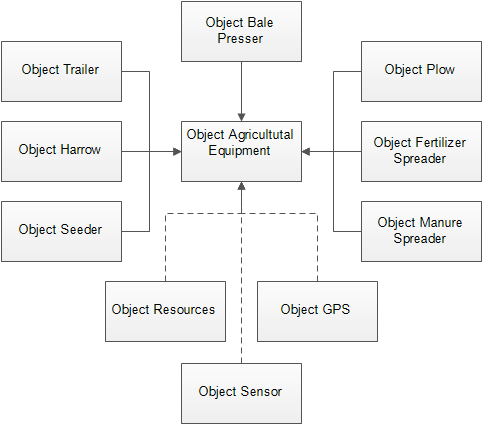
\includegraphics{images/cluster_diagram_agricultural_equipment}
    \caption{}
    \label{fig:cluster_equipment}
\end{figure}

%% structure


%% classes
%% - Definition
%% - Behavioral pattern

\newpage\section{Chapter Summary}
\label{intro_summary}
Through our research in the above sections, we have established a baseline on what a theoretical solution, based on user requirements, might be. To further work towards an end solution, a summation and a look into technological advances in the field is needed, as to better understand the current advances within our problem domain.

Our system definitions act as the establishment of a problem domain, and can be regarded as a rough estimate on what a possible design choice could be. 
The interview has given us an initial list of requirements, that through the use of PACT-analysis can be shortened to the following requirements in the upcoming chapters:

\begin{itemize}
    \item 
\end{itemize}

The context section of the PACT-analysis allowed us to identify external factors that could influence the use of the application, such as weather conditions and internet connectivity.



We have defined our problem domain thanks to our initial contact with the user. The system definitions allowed us to observe the problem domain from different perspectives. After the second interview we found that the first system definition, which focused primarily on being a monitoring and recording tool, was the one that our primary source found most appealing and useful.
Our knowledge from the final system definition was the foundation for our PACT-analysis. This PACT-analysis allowed us to identify the users and their their capabilities and skills as well as several design considerations. One of the considerations is that the users will use the application regularly most of the year, which means that the user will develop a degree of familiarity with the application, thus lowering the demands for immediate usability. The context section of the PACT-analysis allowed us to identify external factors that could influence the use of the application, such as weather conditions and internet connectivity. Lastly the technology section has made it possible to determine design limitations and requirements, such as input- and output-devices.

what we are going to take from this part are the design considerations as described above. As well as the requriemnts given to us by the interview and the technological limitations that a tablet forces us to consider.
The second interview revealed system requirements for the solution, along with identifying the problems our primary source hoped to resolve.



%We can conclude that after the second interview [??] we found the system definition that our primary source found most appealing and useful.

% Defining User Requirements
%  - initial contact and wishes from user
%  - FACTOR-model
% Interview <- analysis of
%  - program requirements
%  - problems
% PACT-Analysis
%  - People
%  - Activities
%  - Context
%  - Technology

%----------------------------------------------------------------------
% Pact analyse 
%   - afsløret ting vi skal lave/undersøge videre
% System definitions
%   - Har enabled os til at se vores problem domain
% Samlet set har alt dette ladet os konstruere en problemstilling bla bla bla.
% Ud fra vores system definition, interview og analyse kan vi konkludere at $manden har et problem, vi har en løsning, der skal samarbejdes og så er alle glade.
\chapter{Technology analysis}
Introduction.
Write things here. \todo{Write actual things here}


\textbf{Fuel efficiency} \newline
In this section we will elaborate on the fuel efficiency of tractors and combine harvesters.
[METATEKST]\todo{write metatext for this}

Tractors
In our studies of the subject we've found that there are many different sizes of tractors, physically as well as in terms of power, and have therefore decided to split them up into three subclasses:
\begin{itemize}[noitemsep]
    \item small tractors (less than 150 bhp)
    \item medium tractors (150-250 bhp)
    \item large tractors (more than 250 bhp)
\end{itemize}
Small tractors have a fuel usage with an average of roughly 20 litres/hour (calculated average of 3 tractors in multiple use scenarios \cite{dlg:case_maxxum_130}\cite{dlg:john_deere_6125R}\cite{dlg:fendt-313-scr}), while medium-sized tractors use roughly 29 litres/hour\cite{dlg:fendt-724-scr}\cite{dlg:claas_arion_650}\cite{dlg:claas_axion_850} and large tractors use 48.5 litres/hour on average\cite{dlg:fendt_939}\cite{dlg:john_deere_8335}\cite{dlg:claas_axion_950}.
Combine harvesters has been more difficult to find exact measures on, we haven't been able to find any specific measures from an independent source, nor was the information available on the 3 manufacturers websites (Claas, Case IH and Massey Ferguson), that we checked, so we will not be able to give an expected average fuel consumption for these.
Another source \cite{erfarland:dieselforbrug} claims that the average field requires 90-100 litres of diesel per hectar in average, and can range from 65-120 litres in the extremes, for an entire season.
Based on the large difference in fuel consumption, found in our research on tractors affected by, amongst others, load, the quality of the surface being driven on, the engine size/power, and the type of work being done, we assume that the fuel economy of combine harvesters will vary in a similar degree. This means that it will be impossible to calculate a single average to be used in lieu of input of historical data from previous years. We have therefore concluded that it will be more useful to allow the user to input their own expected average fuel consumption, if they do not have sufficient data available for the specific field. 


\section{Event Modeling}
Initially the requirements that our contact has specified, in his problem domain, has to be translated into a series of events, that we can later translate into classes that handle objects in a software solution. Hence we will start the process of developing a solution by creating an event list that will depicts the requirements of the given problem domain that the contact has specified he needs solved.

As such, the process of maintaining and running a field, under any given id, has to be split into a series of events that will give us the required data and/or structure needed.

Maintenance of a field can therefore be put into the following events~\cite{lf:korndyrkelse}.

\begin{itemize}[noitemsep]
    \item Field identification
    \item Tilling
    \item Manure spreading
    \item Harrowing
    \item Seeding
    \item Fertilizing
    \item Pesticide spreading
    \item Harvesting
    \item Bale pressing
\end{itemize}

\textbf{Field identification} Is the necessity to know what field the following events are to take place on, and what needs to be done to the current field, as various different crops have different requirements to planting techniques.

\textbf{Tilling} Is the action of tilling the soil, this may, or may not be precedes by stimulating growth to seeds left over from previous seasons of crops.

\textbf{Manure spreading} Is the action of spreading animal fecal matter onto the field. This enhances the soil into fertile soil, which has a higher concentration of fertile minerals and/or chemicals that benefit the growth of crops.

\textbf{Harrowing} Is the action of evening out the field, to prepare it for seeds. this is not a necessary stage, but is recommended to increase the yield and quality of the crops.

\textbf{Seeding} Seeding the field follows the as the next step in growing crops, this is where seeds are applied, at different depths, to the field as to give the specific crop that is grown, the best possible chances to grow into good quality crops.

\textbf{Fertilizing} Is done immediately after the seeds have been planted. This is to give the grops another layer of fertile mineral soil to grow in, and to increase the yield and quality of the crops.

\textbf{Pesticide spreading} Is not done by all field owners, as some farmers prefer to grow their crops without the use of chemicals, using an organic growing technique. However, should the farmer chose to use pesticides, these are only applied to fields with a chance of crop infection, e.g. crickets, flies and/or worms.

\textbf{Harvesting} Requires that the crops on the field are fully grown, and ready to be harvested. There are various different harvesting techniques depending on the crop. However, it is safe to say that some of the crops require that the field is more or less dry, as to prevent the actual yield from the field spoiling before it can be treated for preservation.

\textbf{Bale pressing} Is only required when the crops leave a byproduct such as straw. This is most commonly done by pressing straw into rectangles, after the straw has dried for a period of time, dependent on the weather conditions in the region.

These different events can be solved by using different objects, such as \textbf{Tractors}, which can be defined into a class of vehicles. Those tractors need \textbf{Drivers}, \textbf{Field equipment} and \textbf{Fuel}, which can all be defined in the classes \textbf{Labor}, \textbf{Equipment} and \textbf{Resources}. This gives us the possibility to make an event table, where we can crosscheck the different classes, and objects, with the different events that needs handling. This gives us an excellent tool to get an overview of the complexity of our problem field, and a resource to continue towards a solution to that problem field.

\begin{table}[H]
    \centering
    \begin{tabular}{|l|c|c|c|c|c|c|}
    \hline
         Event/Class & Field & Resources & Equipment & Vehicles & Labor & Yield \\\hline
         Field identification & x &   &   &   &   &   \\\hline
         Tilling       & x &   & x & x & x &   \\\hline
         Manure        & x & x & x & x & x &   \\\hline
         Harrowing     & x &   & x & x & x &   \\\hline
         Seeding       & x & x & x & x & x &   \\\hline
         Fertilizing   & x & x & x & x & x &   \\\hline
         Pesticide     & x & x & x & x & x &   \\\hline
         Harvesting    & x &   & x & x & x & x \\\hline
         Bale pressing & x &   & x & x & x & x \\\hline
    \end{tabular}
    \caption{Event Table}
    \label{event_table}
\end{table}

As seen in \ref{event_table} different classes have been applied to solve the events that we know has to take place to sustain a field and grow crops. Here the "x"'s represent the interaction between the event, and the classes that help solve the specific event, and hence how the classes have an impact on the problem field. Next step is to determine the behavior between the different events and classes.


\begin{table}[H]
    \centering
    \begin{tabular}{|l|c|c|c|c|c|c|}
    \hline
         Event/Class & Field & Resources & Tending & Vehicles & Labor & Yield \\\hline
         Field identification & + &   &   &   &   &   \\\hline
         Tilling       & + &   & * & | & | &   \\\hline
         Manure        & + & * &   & | & | &   \\\hline
         Harrowing     & + &   & * & | & | &   \\\hline
         Seeding       & + & * &   & | & | &   \\\hline
         Fertilizing   & + & * &   & | & | &   \\\hline
         Pesticide     & * & * &   & | & | &   \\\hline
         Harvesting    & + &   & * & | & | & * \\\hline
         Bale pressing & + &   & * & | & | & * \\\hline
    \end{tabular}
    \caption{Behavior Table}
    \label{tab:behavior_table}
\end{table}



\section{Operating systems}
In this section we will figure out what OS (Operating System) that are available for tablets nowadays and what makes the individual OS great and/or bad. This section should help us towards picking a final OS on which our application would be developed for. 
A very big part of the tablet is the Operating system (OS). There's quite a bunch of different OS's we will be listing the most popular systems and explain what makes them individually good or bad.

\textbf{iOS}\newline
The most recent version of Apple's iOS as of this time of writing is iOS 10. It is developed by the American hardware \& software manufacturer Apple. iOS is an operating system that is being used by all of Apple's mobile products, such as their iPad and iPhone products. iOS 10 was released September 13th\cite{macworld:iosreleasedate} with much criticism and complaints from apple-fans and critics alike. Apple made a lot of drastic changes to features such as the lock-screen that many users didn't agree with. Looking past the recent criticisms Apple has made a very robust operating system that does everyday tasks quickly and is very intuitive to use. Their main focus has been on usability and useability rather than extendability and customization. It is a closed system, which means that Apple have locked users away from their local file system except for personal files such as photos, videos, music files etc. Because of this, iOS is also almost safe for viruses and hacking attacks, though there have been popping up more and more exploits\cite{xiao:claud} with each iteration of the system. 
From a development standpoint iOS has previously had a relatively high barrier to entry, since you couldn't just freely build software onto an Apple iOS product. You had to have a registered Apple Developer account, where the cheapest version currently is \$99 USD for a years developer membership. But now Apple offer a student programme and anyone with an Apple ID can build and upload an application to their personal iOS device. You won't be able to upload to Apple's App Store without having a registered developer account\cite{apple:developerprogram}. 

% Mål for afsnit.. 
%   - Finde ud af pros & Cons hos de forskellige OS'er
%   
%% Android - (Manufactures (bliver skrevet om i tablet teknologi afsnittet))
\textbf{Android}\newline % bla bla bla. Android has a tendency to name their versions off of candy.
Android has traditionally named their versions after sweets or cakes, which is also apparent in the most recent iteration, Android 7.0 "Nougat", released the 22. of August 2016\cite{android:latest_version}. Android is the most widely used tablet OS in 2016 \cite{netmarketshare:tablet_os}, and furthermore has the second largest diversity of manufacturers (13 and 194 different models in the source \cite{edbpriser:android}), only surpassed by Windows. Android was originally developed by Android Inc, but was bought by Google in 2005\cite{uk.complex:google_buys_android}, and has been continually developed by them since then. Android is known for its increased customizability compared to iOS
%% Windows tablets 
%( Acer Aspire Switch 11V
%  Asus Transformer Book T100HA
%  Dell Latitude 13 7000 series 2-in-1 (7350)
%  Dell Venue 8 Pro 3000 series
%  Getac F110
%  Lenovo IdeaPad Miix 700
%  Microsoft Surface Pro 4
%  HP Pavilion x2
%  HP Spectre x2
%  Kilde: http://www.pcmag.com/roundup/310159/the-best-windows-tablets
%)
\textbf{Windows}\newline
October 21st 2010 Microsoft released their first iteration of their current attempt into the smartphone market, called Windows Phone 7.\cite{techradar:winphone7_releasedate} With an incredibly tough competition at the time when iOS4 and Android 2.3 "Gingerbread" it performed fairly well. Microsoft made a very robust system with minimal crashes and slowdowns, this 
% Summarization.
% Linux - (???)
% Blackberry (is it even still relevant? - was it ever?)




\section{Sensors}

In this section we will elaborate on some of the currently used sensors and systems in the agricultural industry. We have written this section to define, and gain a basic understanding of, the input data that is currently available in the agricultural industry \cite{sensor:jd_sensors}. But first it should be said that the individual users have varying sensors available, so not all will have the mentioned sensors. \newline

%\textbf{Near infrared sensor}

One of the sensors that is currently present in the agricultural industry is the near infrared sensor. This sensor is used for analysing the constituents of manure, crops, silage and various other organic materials. It does this by exposing the material to near infrared light and analysing the refracted light\cite{sensor:manure-sensor}\cite{sensor:brochure}\cite{sensor:constituent}. \newline
Which is interesting for us because it would allow the user to gain a overview of the quality of the input and output on the field. That data could be used to allow our application, to make better predictions on the expected quality of the output of the fields, based on the input. \newline

%\textbf{Liquid level sensors}

Another relevant sensor, that is used to keep track of fuel consumption, is the  liquid level sensor. This sensor is used for analysing the liquid level in a container. It does this by implementing some reed switches in the container, when the reed switches gets exposed to a magnetic field they react. The magnetic field we want to observe is emitted by a ring magnet mounted on a float. By determine what switches are affected by the floating magnet, the fluid level is determined\cite{sensor:reedswitch}.\newline
Which allows us to get a reading of how much for example fuel a given tractor has consumed in the proses of plowing the field. Which would allow us to make a statistic of how much of a given liquid is used when doing a specific task. \newline

%\textbf{GPS}

GPS is also used in the agricultural industry. Essential to GPS are the satellites floating around earth. At all times at any position you should be in range of at least four satellites. Each of those will be sending their position and time of sending, constantly. The receiver then calculates your distance to the satellite, by comparing its internal time and the time sent by the sent by the satellite. By calculating the distance to the satellite you know you are somewhere in a sphere around the satellite. By finding the intersection between all of the spheres, the position of the receiver is found. This is refereed to as trilateration \cite{sensor:gps}\cite{sensor:gps_physics}.\newline
This is interesting for us because it could be used track the movement of tractors and other machinery. By knowing the position we can for example see what vehicles are used for what work on what field. \newline

%\textbf{Material flow sensors}

Material flow sensors is another sensor currently used in the agricultural industry. This sensor is used for analysing the flow of a liquid through a pipe. There are many different types that all archive the same goal. For example ultrasonic sound can be used to detect this, it works by sending ultrasonic sound waves against and with the flow of the pipe. Sound moving against the flow will travel slower, so by compering the travel time of both its able to determine the speed of the liquid inside the pipe. When you have the speed of the liquid you it simply needs the diameter of the pipe, to calculate the volume of whatever liquid moving though the pipe\cite{sensor:ultrasonic}.\newline
This will in combination with GPS give us a way to track where something like manure or pesticides is applied and the density within a certain area. \newline


\section{API's}
\label{api}
\begin{itemize}[noitemsep]
    \item asd1
    \item asd2
    \item asd3
\end{itemize}
What is an API?
An API is like a library for programmers. A good API will make it possible for the programmer to use certain functions or procedures from a different application without understanding the underlying implementation or structure of this different application.

More to come…
%%\url{https://en.wikipedia.org/wiki/Application_programming_interface}


Which APIs would be interesting in respect to our project
An interesting API which is relevant for our project is the John Deere’s Agricultural API called MyJohnDeere API.
The MyJohnDeere API mentions on their website that their API is capable of providing information such as:
Transfer Data, Agronomic Data, Field Condition, Machine Monitoring, Logistics Data.

When you are using John Deere equipment and you’ve completed a field operation, documentation is sent to John Deere Operation Center. Most of the data that can be retrieved from their API is from this Operation Center.

It is possible to retrieve information about specific costumers, but keep in mind that it is not possible to retrieve information about any costumers without being granted permission. 
Another Note: An EIC license is required to decode display data. So in order to use MyJohnDeere API fully, such a license is required.
Quote
“Note: When an app is connected to this API in Sandbox, only users within the app team will be able to successfully call the API. Users outside of the app team who use the application to call the API will receive a 403 Error.”

% Comments

\section{Statistics}
%%In this part we will look at statistics as well as to look at different formulas and application. furthermore we will look at the state of the art programs that apply these statistical calculation such as excel and mathcad ? 

%%skal være en omkring normal statestik og ikke hardcore gym/uni niveau 
statistics is the science of finding significant trends and deviations from a given set of data either grouped or non-grouped. In this part we will look at different statistical concept such as middle value, spread, variant and graphs derivations. 

%basic terms 
a basic concept of statistic is the observation. An observation is simply the set of samples we want to calculate on in our statistical investigation. The total number of samples in a set is typically described as \(n\). With our set, we can calculate the percentages the frequency of a give sample is of a set. We calculate the percentile frequency by the formulae: 
 
\[ p_i = \frac{f_i} {n} \]
 
where \(p_i\) is the percentage of sample \(i\) and \(f_i\) is the frequency of sample \(i\). The accumulated percentile frequency is simply the sum of all the percentile frequencies going from smallest to biggest sample.

\[ (acc.\ p)_i = p_1 + p_2 + ... + p_{i-1} + p_i = \sum\limits_{a=1}^i p_a \]

What we have been working with until now is called non-grouped observations. That is the set is just raw numbers without any manipulations done. non-grouped observation is preferred when we have a small number of samples in a set, and the samples appear multiple times, any. We can group the non-grouped observation but the data would not be nearly as detailed as it would otherwise. When we, on the other hand have a lot of samples, or the samples predominately have the frequency 1, we would get more details out of the data if we grouped the set in intervals. With grouped observation we introduce two new terms: interval frequency and interval percentile frequency, the former is the number of times that interval occurs, the latter is the percentile occurrences of the interval. 
An non-grouped observation is easiest to visualise in a bar chart whereas a grouped observation is easiest visualised in a histogram. A bar chart is where the name of the samples is out on the x-axis, and the frequency is out on the y-axis, the namesake of the chart will then visually represent the frequency of a given sample. A histogram are very similar to the bar chart but can only be done on a grouped observation. sometimes there will not be a y-axis on a histogram but a legend in the corner where an area is shown and a number in the area which shows the percentage that area represents, the total area of the bars/pillars of the histogram should be 100\%  

to give an example of the above:

    In a class we are interested in finding the age and the high of the pupils. the result where as follows:
    
    \begin{table}[H]
        \centering
        \begin{tabular}{r l c c c c c c c c c }
            Age =& \{14 & 14 & 14 & 15 & 15 & 15 & 16 & 16 & 16 & 13\} \\
            Height =& \{165 & 166 & 170 & 150 & 167 & 180 & 172 & 155 & 177 & 181\} \\
        \end{tabular}
    \end{table}
    
    the total number of samples in each set is n = 10
    we keep the age set as non-grouped and group the height set with interval length of five:
        
        \-\hspace{2cm} height = \{[150], [155], [165, 166, 167, 170], [172], [177], [180, 181]\}
        
    the frequency of 14 is 3, and to calculate the percentile frequency of 14 we use the formulae
    
        \[p_{14} = \frac{f_{14}} {n}\]
        
    which is 
    
        \[30\% = \frac{3} {10}\]
        
    the interval frequency of [165,170] is 4 and we calculate the percentile interval frequency in the same way as the percentile frequency 
        
        \[40\% = \frac{4} {10}\]
    
    to find the accumulated percentile frequency we simply add all the percentile frequencies together, this will often be 99,9 or 100,1 this discrepancy is caused by round errors.
    
    a bar diagram of the age set would look like:
    
    \begin{figure}[ht]
    \centering
    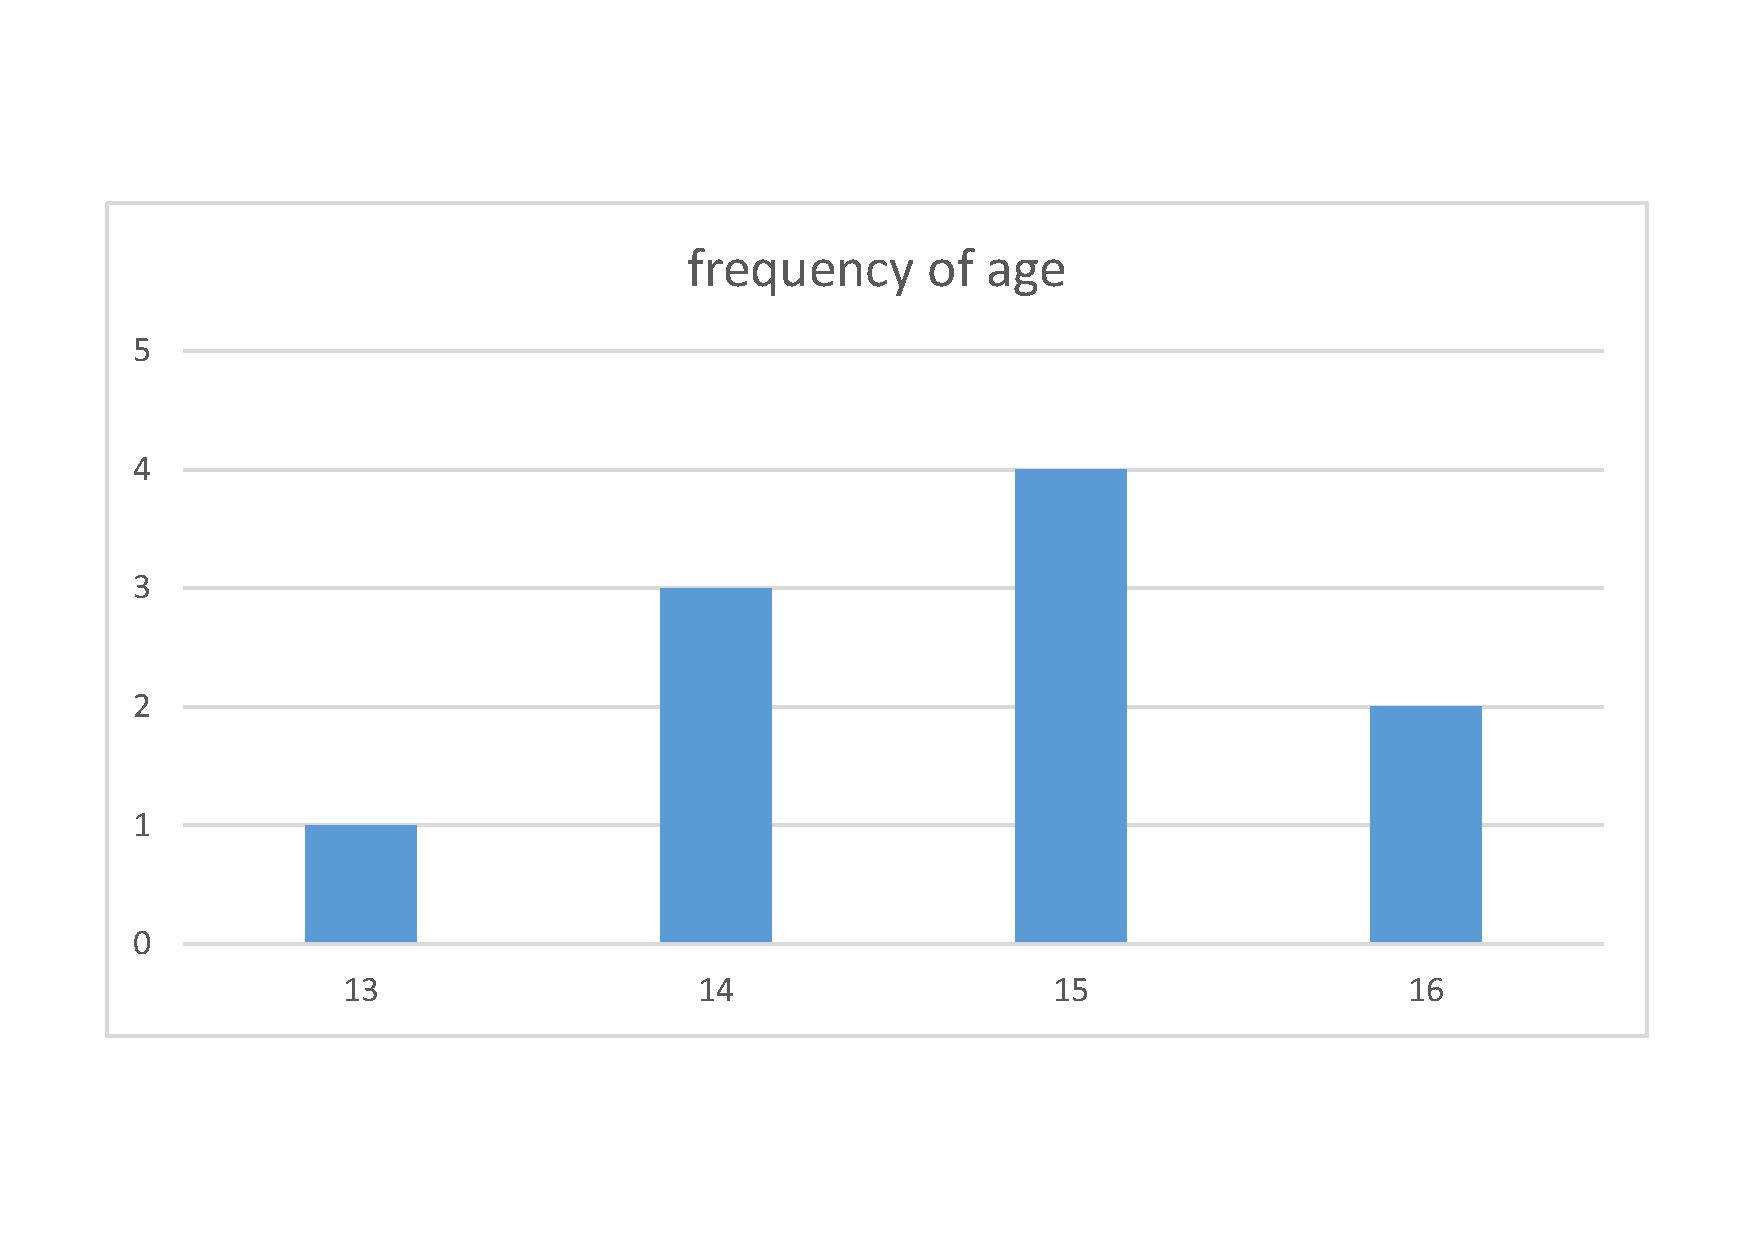
\includegraphics [width=12cm]{images/Frequency_age.pdf}
    \caption{}
    \label{fig:frequency_age}
    \end{figure}
    
    a histogram of the height set with a y-axis would look like: 
    
    \begin{figure}[ht]
    \centering
    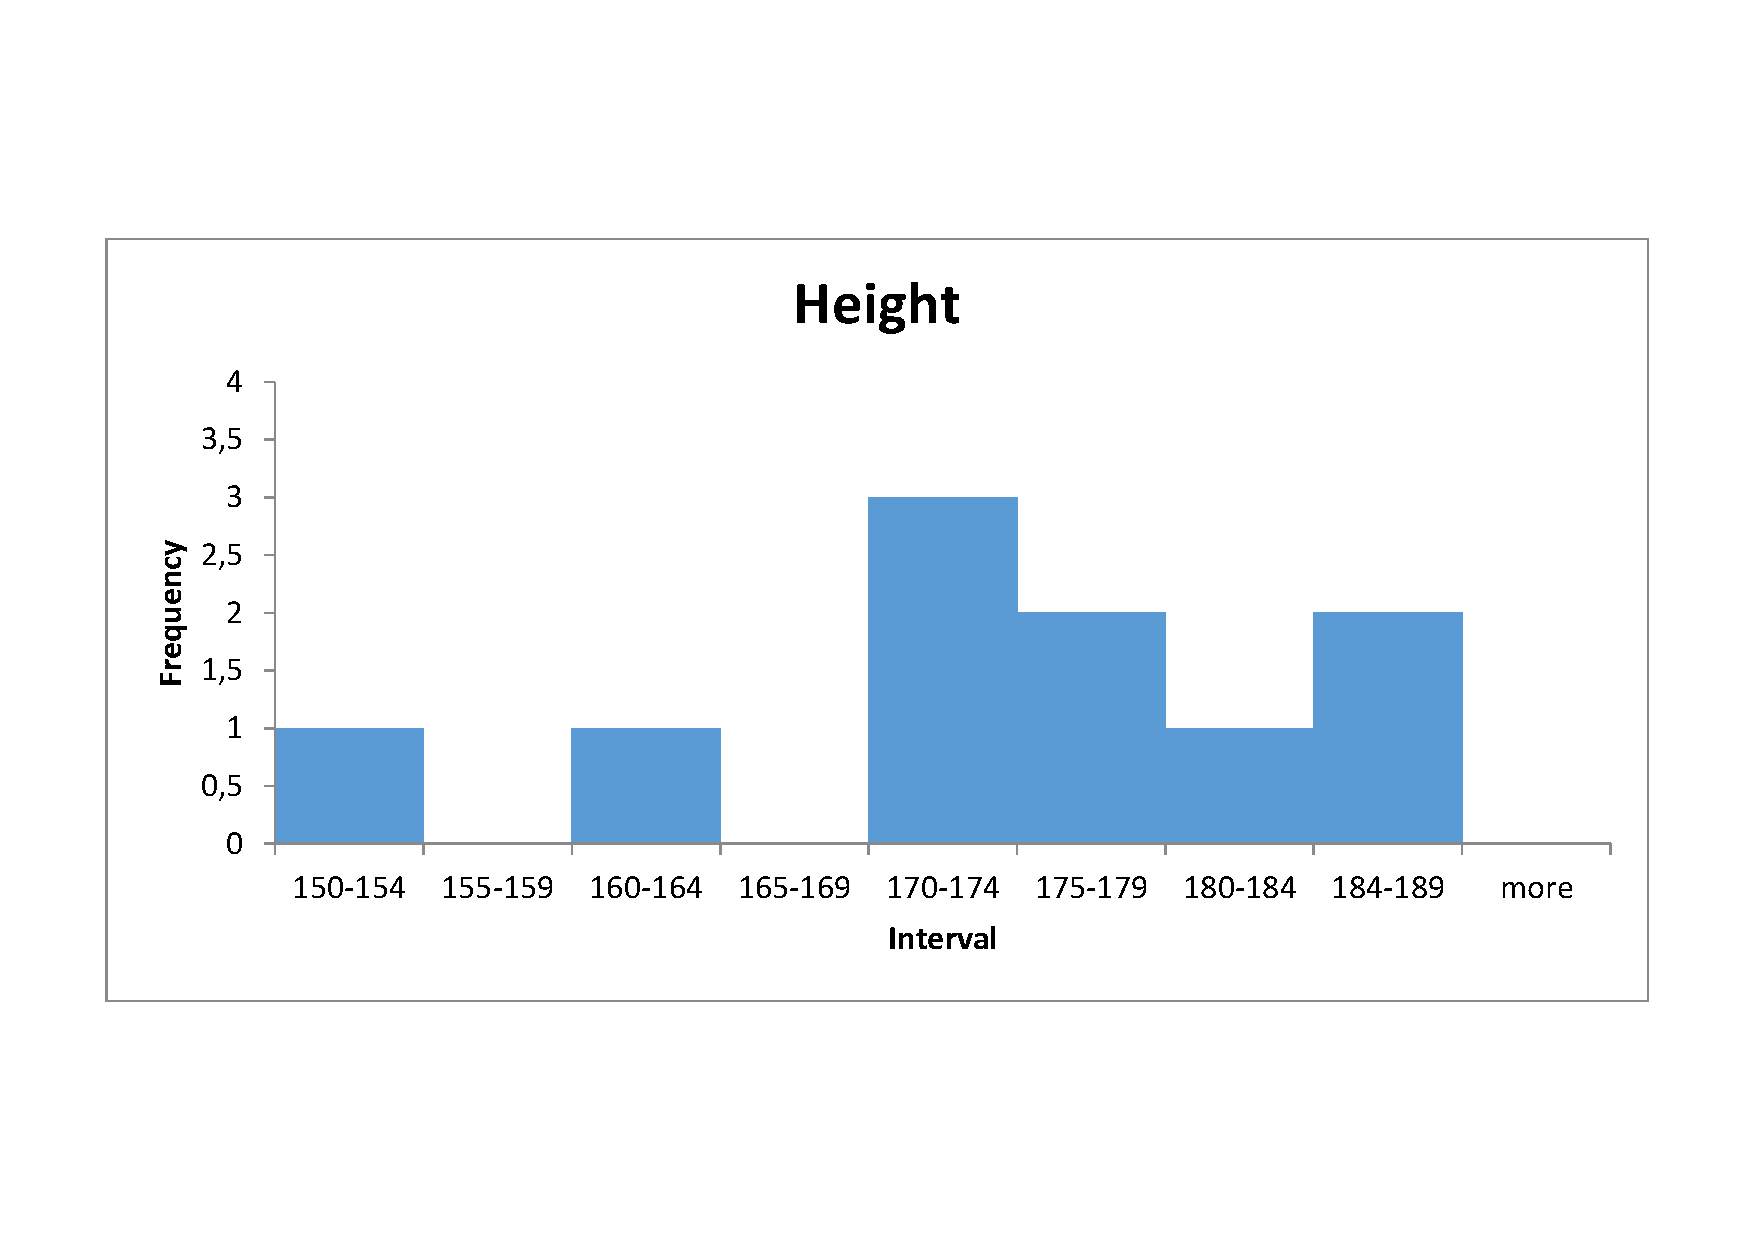
\includegraphics [width=12cm]{images/Height.pdf}
    \caption{}
    \label{fig:Height}
    \end{figure}
    
The Median, is the sample that separates the upper values from the lower value in a data set. in a 7 sample data set with rising values the median is quite simply the 4Th sample. If there is an equal number of sample the median is calculated by taking the sum of the two numbers in the middle and divide it by 2. 

The mean, or the average, on the other hand are quite simply the average of the sum of all the samples in a set and denotes by \(\overline{x}\). to calculate the mean we simply multiply the frequency with its sample and take the sum of the multiplications, we then divide the sum with the total number of samples. 
this gives us the formulae: 

\[ \overline{x} = \frac{1}{n} * \sum\limits_{a=1}^i f_a * x_a = \frac{f_1 * x_1 + f_2 * x_2 +...+ f_i * x_i}{n} \]    
    
where \(x_i\) is the iTh sample.

we can also calculate it from the frequency with the formulae: 

\[ \overline{x} = \sum\limits_{a=1}^i p_a * x_a = p_1 * x_1 + p_2 * x_2 +...+ p_i * x_i\]

We can't do the same with a grouped observation. This is because we can't multiply the value of the sample with the frequency because the samples are the whole interval and not just one value. 
we need to first find a median-value for the interval from the start \(a\) to the end \(b\) we find this by taking the sum of \(a\) and \(b\) and divide with 2, or in other words: 

\[ m = \frac{a+b}{2}\]

to then find the mean we simple change out value \(x\) with the median-value \(m\)

now that we have found out how we calculate the mean we can find out the variance and spread. the variance we calculate by finding the distance between the set and the mean value square it and find the average of it, or in other words

\[Var(x) = \frac{1}{n} * \sum\limits_{a=1}^i f_a *( \]




%% SOLUTION SPACE %%
\part{Solution} % placeholder navn

\chapter{Design}
%\input{solution/design.tex}

\chapter{Implementation}
%\input{solution/implementation.tex}

\chapter{Test}
%\input{solution/test.tex}

\part{Evaluation and further work}
%\input{taxonomy/taxonomy.tex}

\chapter{Appendix}
Raw untranslated transscript of interview with Jens-Ole Larsen performed by interviewer Mikkel E. Holm.
The interview is line seperated, and each line denoted with abbreviated name of interviewer and interviewee, as seen below:

\begin{longtable}{ r | p{13.5cm} }
    MEH & Mikkel Elkjær Holm\\
    JOL & Jens-Ole Larsen
\end{longtable}

% Ny table of pleasure and satisfaction
Phone interview at 2016-09-30 12:31, length 12m 46s.
\label{transscript:jens_ole}
\begin{longtable}{ r | p{13.5cm} }
    JOL & … Bluetooth, så man kan hele tiden tage dataen ud, så der .. hvis der/det var noget hvor at man kunne sige at det her det ville være kanon, så kan man have en tablet, med det her program på, og så integrere med de enheder man havde, ik.\\
    MEH & Ja.\\
    JOL & alt hvad der hedder gps, det ville jo være via den her tablet, så det behøver man ikke at integrere sådan hvor er du henne i verden\\
    MEH & nej ikke inde i .. øh\\
    JOL & ... ja det vi jo kunne gøre i den enhed .. tablet, det faktiske input vi skal have det er fra udbyttemåleren fra såmaskinen – hvor meget sår vi ud\\
    MEH & ja\\
    JOL & Og så ville vi kunne danne en komplet .. øhm.. \\
    MEH & altså en komplet løsning til det? \\
    JOL & .. en komplet kalkulation, og så kunne man jo også gå et skridt videre, og sige at den enkelte landmand der egentlig ikke bruger maskstationen, så har han det program og .. og.. og det program det gør jo at hvis vi så kører for den landmand, så skal vi jo egentlig bare logge på hans, eller overføre dataen fra hans .. \\
    MEH & ja, fra hans system \\
    JOL & ... ja \\
    MEH & ja, lige to sekunder.. så .. øh .. så det du søger efter det er en komplet pakke med det hele, hvor vi binder alle de her \\
    JOL & .. ja en {uforståeligt} Seges, så har de {??} online, og der findes også en app der hedder ”Marktracking”, eller ”Marktracker” eller sådan noget, {??} de her markblokke og .. og hvad det hedder .. elektronisk, for det er jo til gengæld gennem EU, fordi det er på den måde at man får øhm .. EU-støtte på{?} \\
    MEH & Ja, det er den nye lov-ting øhm.. \\
    JOL & jaja, jaja, som de har til deres traktorer, og det gør jo så at i det øjeblik at vi kommer med en {??} indenfor den der {??} traktor, så slipper de øhm .. ikke .. så taber de tråden {?} så får de {lækre pletter?!?} \\
    MEH & nej, øhm .. og de platforme de .. sådan noget.. hvad er det (red. for) nogen systemer de kører på de her .. er det telefoner, eller tablets eller .. \\
    JOL & .. jamen dem der findes i dag de sidder på traktoren \\
    MEH & i traktoren? \\
    JOL & .. ja, så skal du trække det ud, via USB eller et eller andet big data, og der mener jeg i hvert fald at man skal tage tabletter og integrere med den enhed der køres, sådan så når nu man har en tablet med, og er ude og køre, så sætter man USB-stikket i, og så vælger man at det her er en John Deere (red. Traktorproducent) og så .. så.. og det er selvfølgelig ikke noget man kan ødelægge sådan lige ved at {utydeligt}\\
    MEH & grin .. ja, jaja \\
    JOL & {utydeligt} hvis nu man udvikler bare til én type maskiner, ik’, så vil man jo .. så vil de andre i det her .. i det øjeblik at de skal til at betale for at få det {utydeligt} \\
    MEH & ja, jaeh .. øhm ja .. nu skal jeg lige ... du kommer jo langt omkring, så jeg er lige nødt til at springe nogle spørgsmål over .. jeg skal lige se \\
    MEH & jaja, jo tak, heh .. øhm.. nu skal jeg lige se .. øhm .. og ja .. jeg kan egentlig bare lige rykke ned her til de .. til de lukkende spørgsmål .. øhm .. for eksempel den der tablet .. hvad forestiller du dig at det skal være for en type.. bare en ganske normal en .. en iPhone .. nej, en Apple eller .. \\
    JOL & .. vi bruger .. vi bruger jo bare Apple .. og vi bruger jo også Android, ik’ .. men .. øh .. men-men-men min .. {utydeligt, måske noget med ”min holdning er”?} der er Apple .. det er ikke brugbart, fordi vi har en masse excel, og efterbehandling og sådan noget \\
    MEH & ja \\
    JOL & .. og vi har ikke andet en bøvl med det der integration lige så snart det er over (red. Et) Apple-produkt det er fint nok når man har noget der fuldstændig er gemt \\
    MEH & ja .. ja okay \\
    JOL & .. så er der ikke noget \\
    MEH & nej så er det ikke .. \\
    JOL & ind .. indover Apple, men lige så snart du får tredjepartsprogrammer .. \\
    MEH & ja .. ja, selvfølgelig, selvfølgelig \\
    JOL & så.. så har man ikke andet end bøvl med .. \\
    MEH & ja, med Apple \\
    JOL & .. ja med Apple \\
    MEH & det .. øh .. det kender vi godt .. øhm .. ja .. øhm .. ja.. jeg.. jeg tror at vi har været omkring det (red. Hele) .. hvad det var vi ville spørge om .. og det  \\
    JOL & .. nåh.. det var sgu da meget nemt  \\
    MEH & ja ..heh.. det er jo .. sådan lidt .. øhm.. vi har fået noget information om sådan hvordan vi skulle lave sådan nogle spørgsmål {utydeligt}.. så, men øh.. nu var vi så meget omkring det her helt i starten .. helt bare her med det første spørgsmål, så det er bare super-fedt .. øhm .. (Asger siger ”Spørg om der er {utydeligt} .. telefonen) .. ja? \\
    JOL & .. men det der .. øhm .. i kan jo sætte jer ned og så tænke jer .. er det muligt og så gå ind og kigge på .. så vil jeg gå ind og ringe til Seges og {utydeligt} .. for det og det.. og at i tænker i de der baner, ik’ \\
    MEH & jo \\
    JOL & for at se hvordan får i fat i de kort der, det kan godt være .. det kan godt være at de har et program til rådighed til at videreudvikle, det skal jeg ikke kunne sige. \\
    MEH & ja .. nej \\
    JOL & og så kan i .. sådan lige gå ind og kigge i øhm .. i en maskineforhandler, det kan være (red. Massey) Ferguson, eller være et eller andet andet produkt og sige .. hvordan .. hvordan flytter jeg dataen herfra og ud, og så kan det være at de kommer og fortæller jer at der findes også det program, og der findes også det program, og det findes også det program, ik’ \\
    MEH & jo \\
    JOL & .. og så kontrollere lidt .. hvordan virker de der ting, og have det i baghovedet at det skal integreres hele lortet, i et, \\
    MEH & ja .. hehe \\
    JOL & sådan så vi ikke står der. Fordi at nu har vi hele vores maskinpark den består af to typer traktorer og to typer mejetærskere, og så kommer vi over og tager et nyt produkt, ik’ \\ 
    MEH & ja \\
    JOL & .. og så er vi færdige med at bruge programmet \\
    MEH & ja \\
    JOL & ik’ \\
    MEH & jo \\
    JOL & .. og det er jo problemet i dag, fordi vi vil meget gerne have leveret data til landmanden som han kan bruge, enten som en CD eller som at han direkte kan importere et eller andet eller en excel {utydeligt} nu kan jeg {utydeligt} efter det her \\
    MEH & ja \\
    JOL & i mit bogføringssystem \\
    MEH & jo, men øhm .. men øhh.. vi siger mange tak for informationen.. \\
    JOL & .. ja det er sgu da en nem opgave (red. Sarkastisk) \\
    MEH & jaja, herregud, ja det .. (red. Sarkastisk) \\
    JOL & ja, hvis jeg havde tiden gjorde jeg det selv .. haha  \\
    MEH & heh.. det er lige det, ej, øhm.. vi kigger lige på .. det du har sagt til os og øhm.. så hvis vi må kontakte tilbage på et eller andet tidspunkt \\
    JOL & .. du ringer bare.. \\
    MEH & vi ringer bare? Jamen okay .. det lyder godt! \\
    JOL & jah {utydeligt} \\
    MEH & ja, jamen \\
    JOL & .. så finder vi hurtigt et tidspunkt ..\\
    MEH & ved du hvad, det lyder supergodt .. du må .. du må have en fortsat god dag \\
    JOL & .. ja i lige måde da \\
    MEH & jow .. hej-hej \\
    JOL & hej-hej \\
\end{longtable}

\label{appendix_interview}

\section{Coding style}
%\input{appendix/coding_style.tex}
\section{Glossary}
\label{glossary}
\section{Inheritance diagram}

%% APPENDIX SPACE %%
\begingroup
\raggedright
\bibliography{bibtex/litterature}
\endgroup

\appendix
\clearforchapter

\phantomsection
\pdfbookmark[0]{Appendix}{appendix}

\end{document}
